\section{Security Analysis}
\begin{figure}
\centering
\begin{subfigure}{.4\columnwidth}
  \centering
  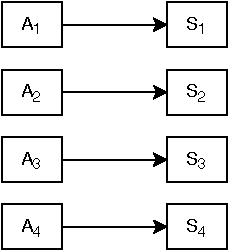
\includegraphics[width=0.8\linewidth]{figures/Set_diagram.pdf}
  \caption{Traditional set index}
  \label{fig:one-to-one}
\end{subfigure}%
\begin{subfigure}{.4\columnwidth}
  \centering
  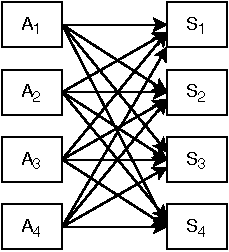
\includegraphics[width=0.8\linewidth]{figures/many-to-many.pdf}
  \caption{Randomized set index}
  \label{fig:many-to-many}
\end{subfigure}
\caption{Set Index}
\label{fig:set_diagram}
\end{figure}
To show the security benefits of our proposed design, we focus on the mapping between the memory address and the set index. With the traditional approach, the attacker can learn the set index bits of the victim's address after finding the conflicting set number with full confidence since the mapping between the original set index and the actual set to which the address is mapped in the cache is one-to-one. However, in our design we provide a many-to-many mapping from the original set index to the mapped set in the cache. Therefore, even when the attacker has learned the conflicting set number, the original index bits are completely unknown because of our hashing schemes. A single static hash scheme alone is capable of hiding the victim's address completely. We add more security on top of this by introducing different schemes at the page level granularity and implicitly changing the hash schemes as described in section X and Y respectively. \\
More formally, we can model the cache side channel as a communication channel and prove that the channel capacity is zero for our proposed design. We assume an ideal case where any cache access made by the victim results in the eviction of an attacker's cacheline due to conflict and is observable by the attacker. The original set number of the victim's cacheline is referred to as the input channel symbol and the conflicting set number observed by the attacker is referred to as the output channel symbol. Let $P(b|a)$ denote the conditional probability that given the input symbol $a$, the output symbol $b$ is observed. Due to the randomness introduced by our hash scheme, $P(b|a) = P(b'|a')$ for any $b$, $a$ and $b'$, $a'$. Using information theory we can easily show that the capacity of such a channel is zero \cite{info_theory}.
